\section{Prediction Evaluation}
\label{sec:experiments}

In previous section, we shown theoretical results with empirical measures  on realization of networks using the generative property of the probabilistic models. In this section, we seek to explain the predictive performance on several datasets by examining their empirical properties and how well the models can capture them. This analysis provide also a study on a systemic comparison of both models, IMMSB and ILFM. Particularly we will see that performance of those models really depend on the type of data we want to fit.

This section is organized as follow In first subsection we described our measure for the preferential attachment effect. In the second we present the synthetic and real dataset that we have used. In the third we present our experimental setting. In the last we report our results.

\subsection{A measures for the preferential attachment effect}

\label{sec:experiments-busrt}
Preferential attachment leads to networks characterized by a degree distribution with heavy tail which can take the form of a power law. To evaluate this property,  we  plot the degree distributions in log log scale for the original network and the generated network. Comparison of the degree distribution with a linear function in the log-log scale  gives us a qualitative measure for the preferential attachment. However, for a better evaluation of the power law behavior of degree distribution we rely on a  goodness a fit based on a Kolmogorov-Smirnov (KS) test. We follow the protocol described in \cite{clauset2009power} which consists of the following steps:
\begin{itemize}
	\item Estimate the parameters $x_{min}$ and $\alpha$ of the power law model.
	\item Calculate the goodness of fit between synthetic datasets generated with the power law and the data. The resulting $p$-values gives an estimates of the          plausibility of the hypothesis for the data.
\end{itemize}

As mentioned in \cite{clauset2009power} high value of the $p$-value should be considered with caution for at least two raisons. First there may be other distribution that match the data equally or better. Second, a small number of samples of the data may lead to high p-value and reflect the fact that is hard to rule out an hypothesis in such a case.

\subsection{Datasets}
In our experiments, we consider four artificial networks and two real networks.\\

\textit{Artificial networks}

The artificial networks have been generated with ANC-Generator \cite{largeron2015}. This generator has been chosen because it allows to build attributed graphs with  community structure faithfully following the known properties of real-world networks such as preferential attachment and homophily.
Moreover, by modifying the parameters, these properties can be weakened. Finally, ANC-Generator is available under the terms of the GNU Public License and the        parameters can be shared for experiments reproducibility.

Four artificial networks have been generated, each one corresponding to a configuration  regarding the properties of interest.
Table \ref{table:artificial_networks} summarizes these four configurations. We report the seed and parameters that we use those synthetic networks in appendix \ref{seed_dancer	}. Each generated networks correspond to a different combination where homophily and preferential attachment are more or less characterizing the underlying networks. For example...

\begin{table}[h] \label{table:artificial_networks}
	\caption{Artificial networks properties.}
	\begin{tabular}{lrrrr}
		\hline
		Networks   &  p-value    &  Modularity & Clustering coefff & density   \\
		\hline
		$Network1$ b/h   & yes &0.59  & 0.06 & 0.007  \\
		$Network2$ b/-h  & yes &0.43  & 0.08 & 0.006\\
		$Network3$ -b/-h & no  &0.71  & 0.49 & 0.01 \\
		$Network4$ -b/h  & no  &0.68  & 0.61 & 0.06 \\
		\hline
	\end{tabular}
	\caption{Real networks properties.}
	\begin{tabular}{lrrrr}
		\hline
		Networks    &  p-value    &  Modularity & Clustering coefff & density   \\
		\hline
		$fb\_uc$          & yes & -  & 0.10 & 0.008 \\
		$manufacturing$   & yes & -  & 0.59 & 0.24 \\
	\end{tabular}
\end{table}

\textit{Real networks}

We evaluate also the models on two  real networks.
The first one \footnote{available at:} is built from an online community of 1899 students from the University of California. Each node corresponds to a user and a    directed edge represents a sent message.
The second one \footnote{available at:} is an internal email communication network between employees of a mid-sized manufacturing company. Each vertex is associated  to an employee and an oriented link represents like previously a sent email.

Table 1 summarizes some properties characteristics of these artificial and real datasets. The  the p-value measure is computed as described in \ref{} as reference for the global preferential attachment effect. we also report the modularity on the a given (true) partition (by Dancer) of the networks, and the clustering coefficient.

\begin{figure}[h]
	\centering
	
	\minipage{0.25\textwidth}
	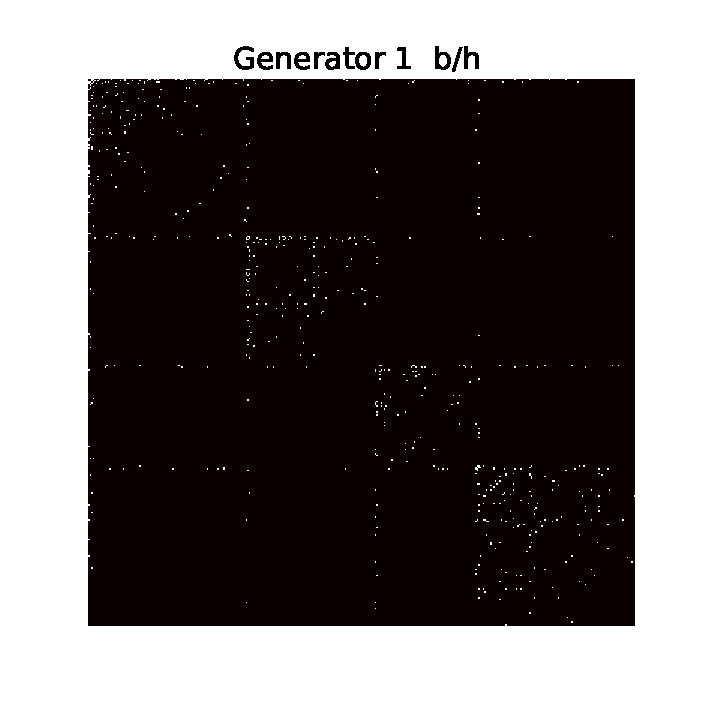
\includegraphics[scale=0.4]{img/g1}
	\endminipage
	\minipage{0.25\textwidth}
	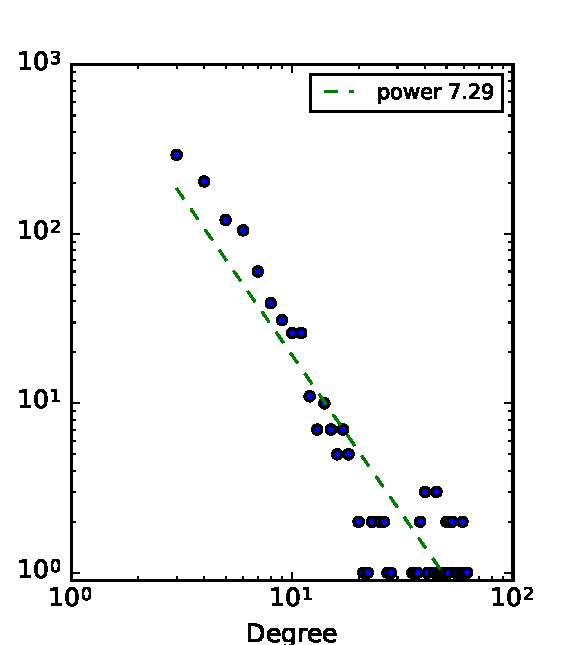
\includegraphics[scale=0.4]{img/g1_d}
	\endminipage
	\vspace{-0.4cm}
	\minipage{0.25\textwidth}
	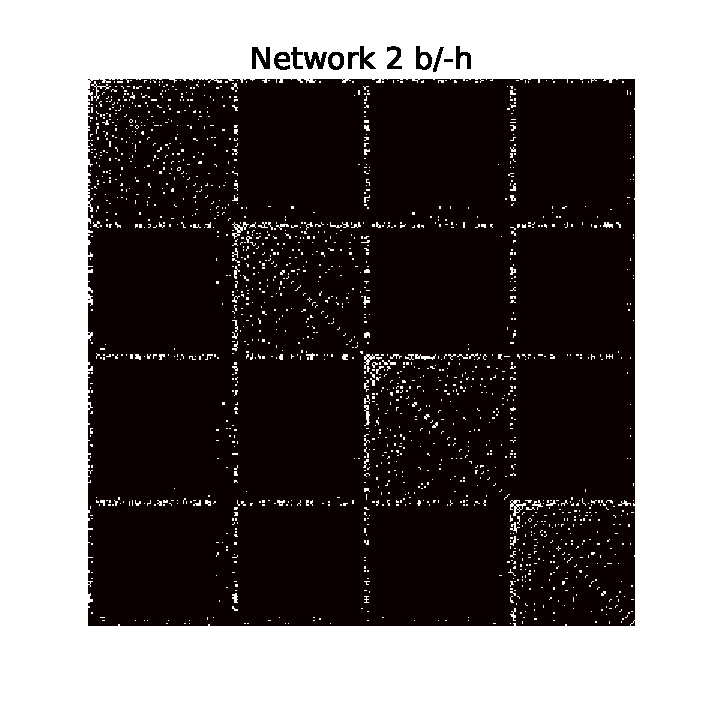
\includegraphics[scale=0.4]{img/g2}
	\endminipage
	\minipage{0.25\textwidth}
	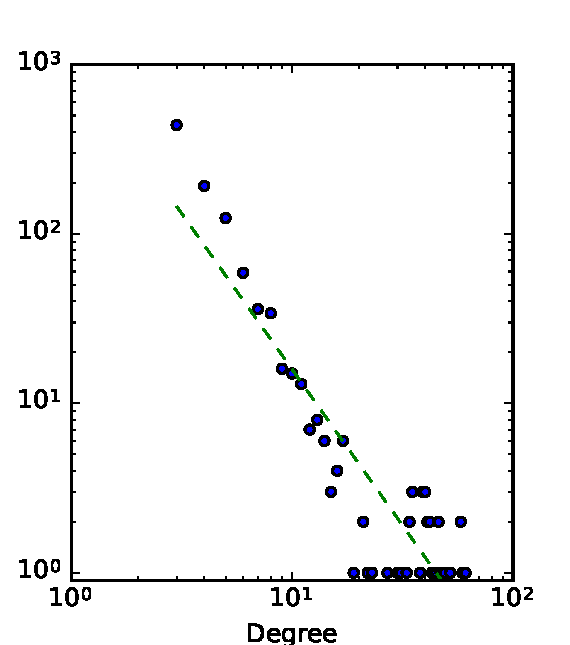
\includegraphics[scale=0.4]{img/g2_d}
	\endminipage
	\vspace{-0.4cm}
	\minipage{0.25\textwidth}
	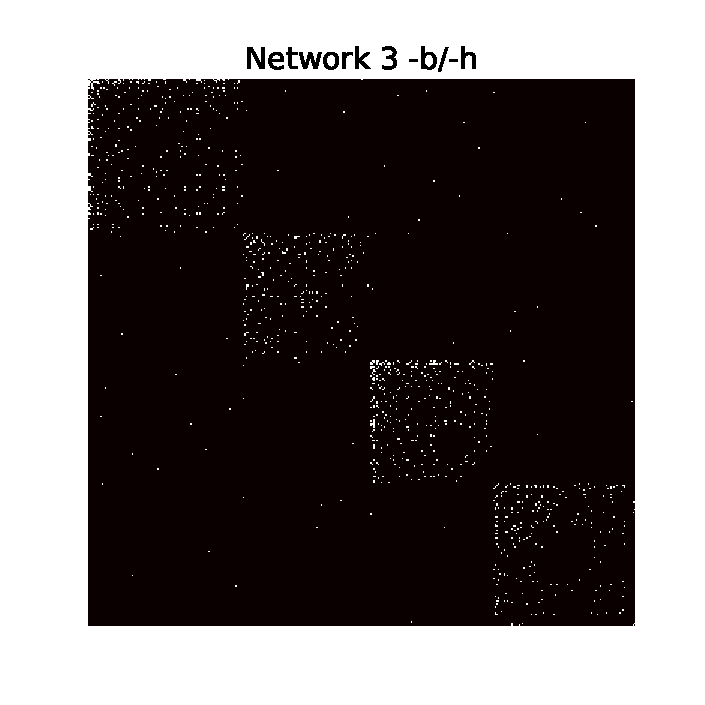
\includegraphics[scale=0.4]{img/g3}
	\endminipage
	\minipage{0.25\textwidth}
	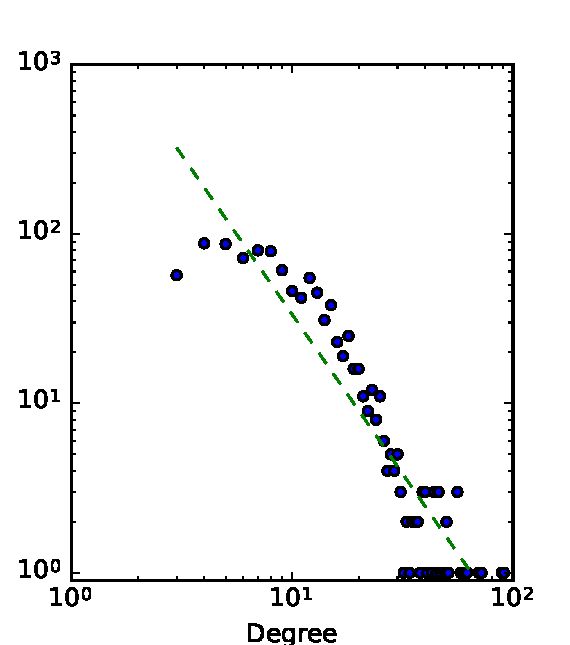
\includegraphics[scale=0.4]{img/g3_d}
	\endminipage
	\vspace{-0.4cm}
	\minipage{0.25\textwidth}
	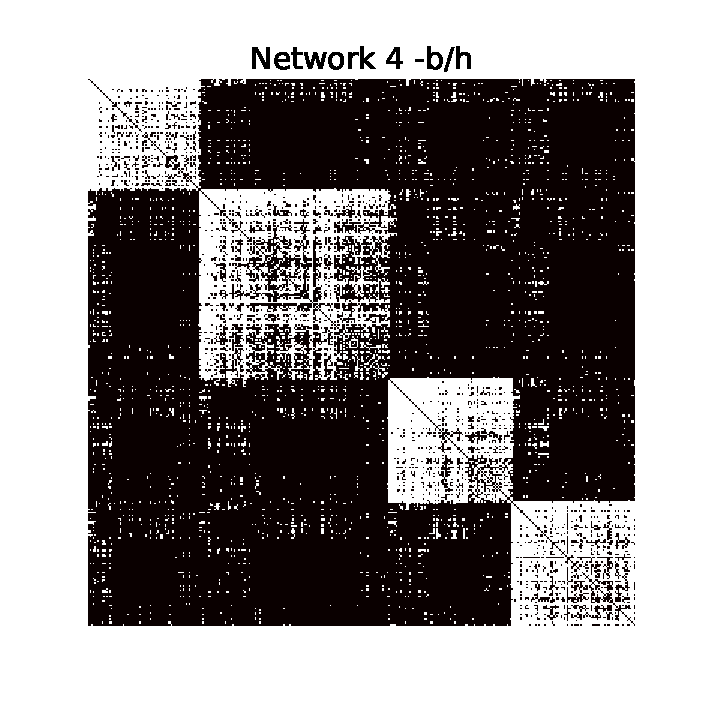
\includegraphics[scale=0.4]{img/g4}
	\endminipage
	\minipage{0.25\textwidth}
	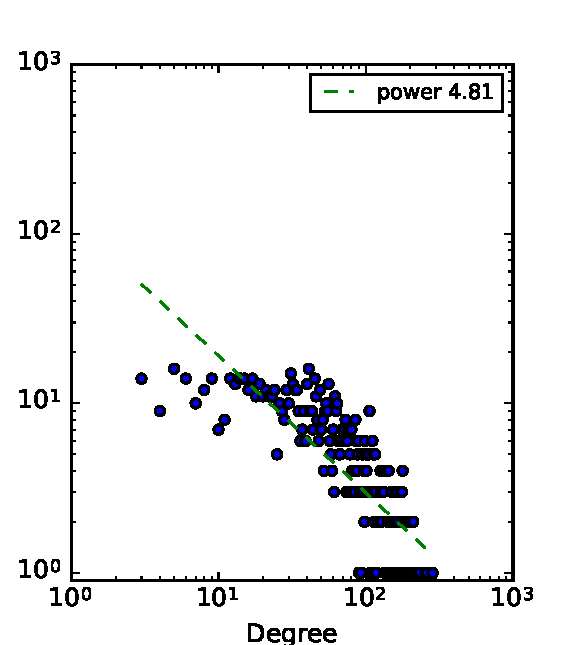
\includegraphics[scale=0.4]{img/g4_d}
	\endminipage
	
	\caption{artificial Networks. (left) adjacency matrix. (right) degree distribution}
	\label{fig:synt_graph}
\end{figure}

\begin{figure}[h]
	\centering
	
	
	\minipage{0.25\textwidth}
	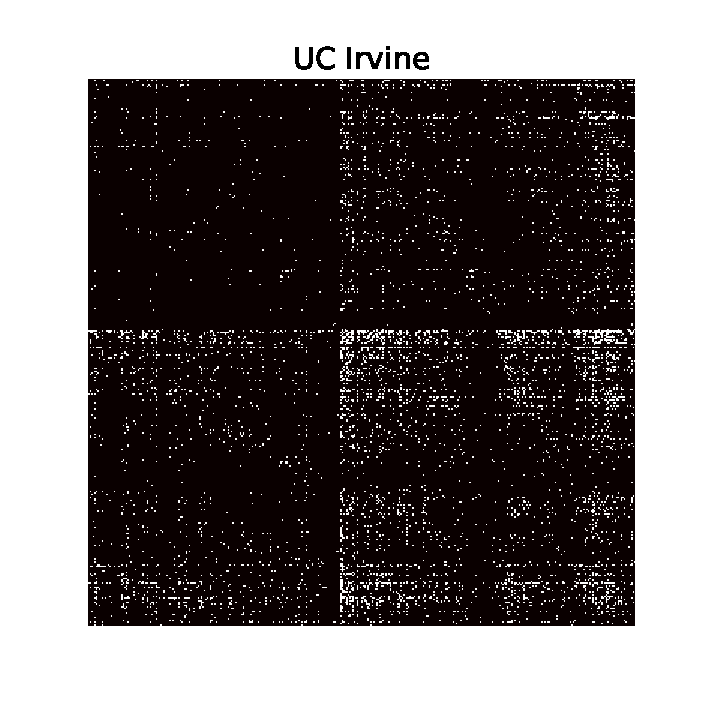
\includegraphics[scale=0.4]{img/irvine}
	\endminipage
	\minipage{0.25\textwidth}
	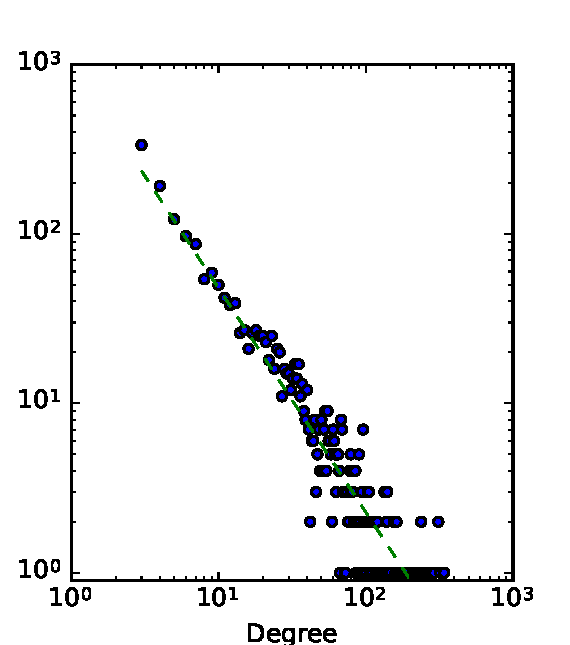
\includegraphics[scale=0.4]{img/irvine_d}
	\endminipage
	\vspace{-0.4cm}
	\minipage{0.25\textwidth}
	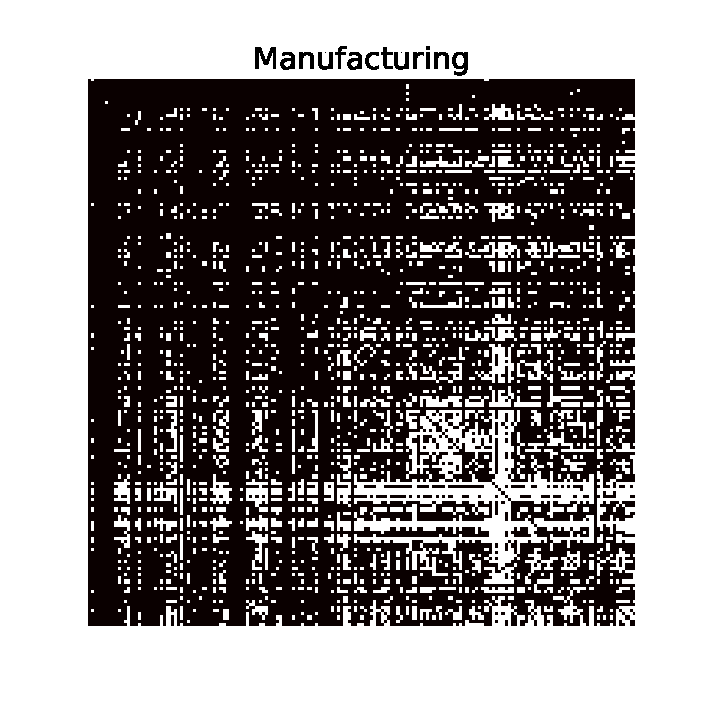
\includegraphics[scale=0.4]{img/manufacturing}
	\endminipage
	\minipage{0.25\textwidth}
	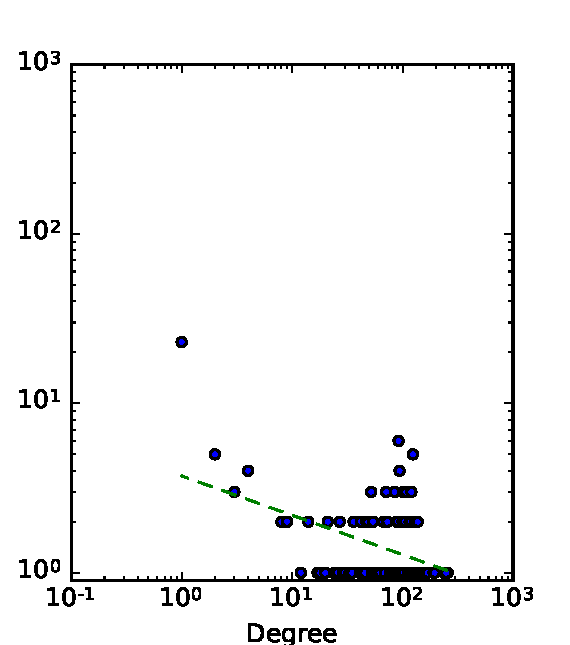
\includegraphics[scale=0.4]{img/manufacturing_d}
	\endminipage
	\caption{Real Networks. (left) adjacency matrix. (right) degree distribution}
	\label{fig:real_graph}
\end{figure}



\subsection{Experimental Settings}
For each datasets described,  we run a MCMC inference consisting of 200 iterations to learn the posterior distribution of each the IMMSB model and ILFM, described in \ref{sec:models}. For IMMSB, concentration parameters of HDP were optimized following \cite{HDP} using vague gamma priors $\alpha_0 \sim \text{Gamma}(1,1)$ and       $\gamma \sim \text{Gamma}(1,1)$. The parameter for the matrix weights were fixed to $\lambda_0=\lambda_1=0.1$. For ILFM, the IBP hyper-parameter was fixed to   $\alpha=0.5$ and the weights hyper-parameter to $\sigma_w = 1$. Each experiences were averaged on 10 repetitions, and results were found to be stable regarding on the random  initialization and stochastic optimization.


We evaluate the performance prediction of the models by building a training set and a testing set from the original datasets. In order to achieve this we build a random mask consisting of 20 percent of the size of the adjacency matrix. This mask is used a our testing set, while the 80 remaining percent are used as a training set.

In figure \ref{fig:auc} we report the Area Under Curve for for each datasets in order to compare the behavior of IMMSB and ILFM. In figure \ref{fig:gen_graph_s} and \ref{fig:gen_graph_r} we used the models learned on the training set to generate a full networks and report the global and local degree distribution. Finally we report a detailled table on precision and recall for each experiment that corroborate the AUC report in annexe \ref{sec:precision_recall}.

\begin{figure}[h]
	\centering
	
	\minipage{0.25\textwidth}
	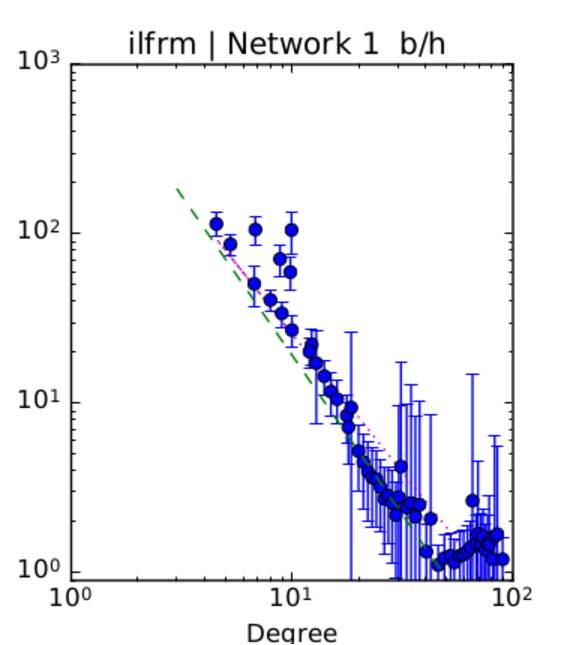
\includegraphics[scale=0.4]{img/ilfrm_g1_d}
	\endminipage
	\minipage{0.25\textwidth}
	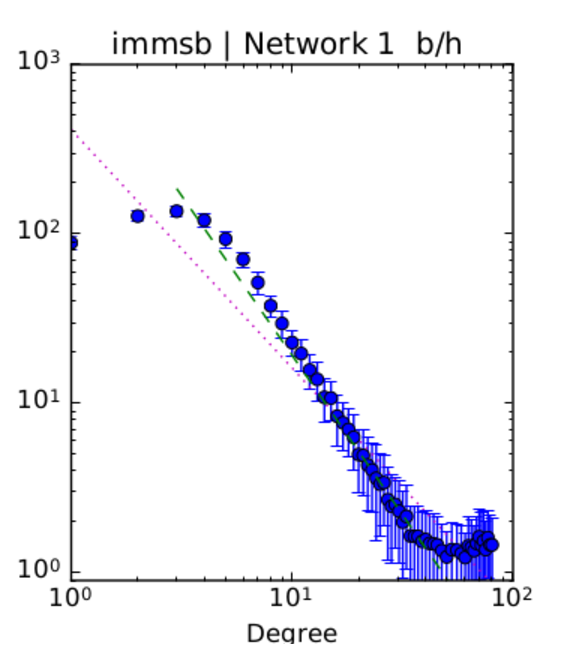
\includegraphics[scale=0.4]{img/immsb_g1_d}
	\endminipage
	\vspace{-0.4cm}
	\minipage{0.25\textwidth}
	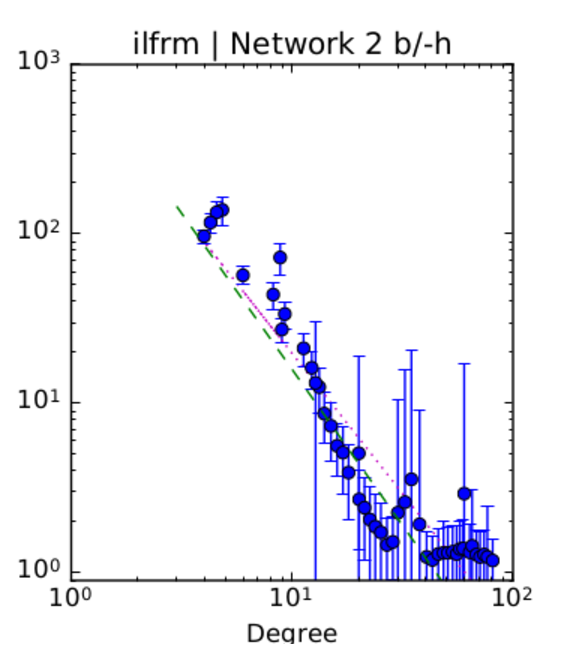
\includegraphics[scale=0.4]{img/ilfrm_g2_d}
	\endminipage
	\minipage{0.25\textwidth}
	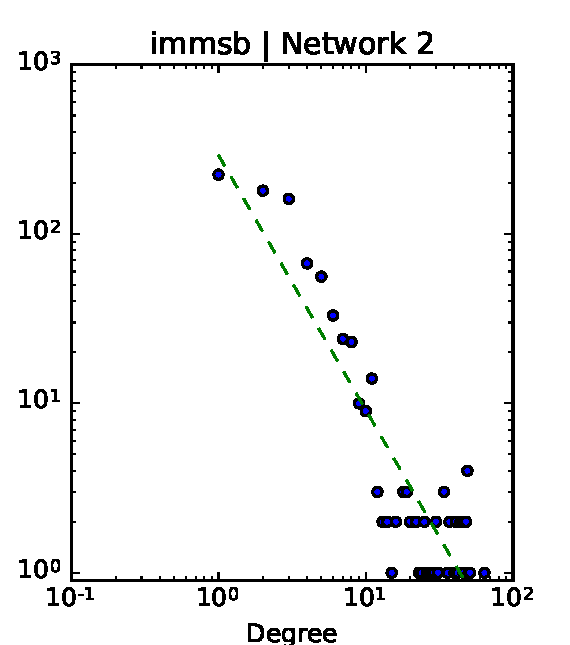
\includegraphics[scale=0.4]{img/immsb_g2_d}
	\endminipage
	\vspace{-0.4cm}
	\minipage{0.25\textwidth}
	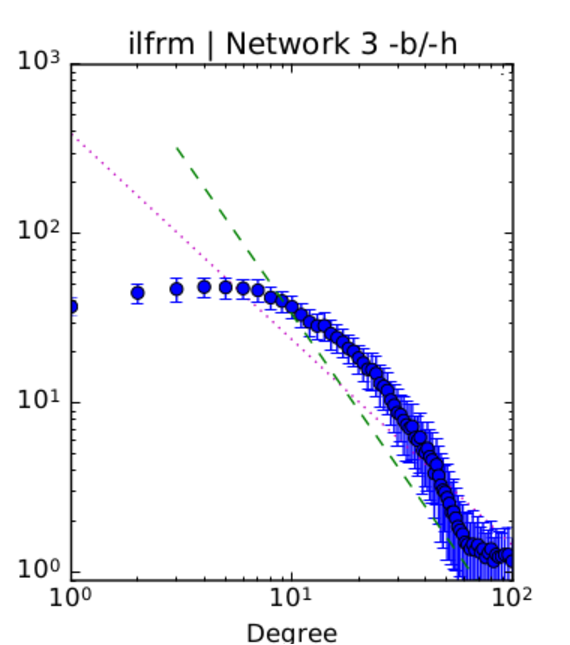
\includegraphics[scale=0.4]{img/ilfrm_g3_d}
	\endminipage
	\minipage{0.25\textwidth}
	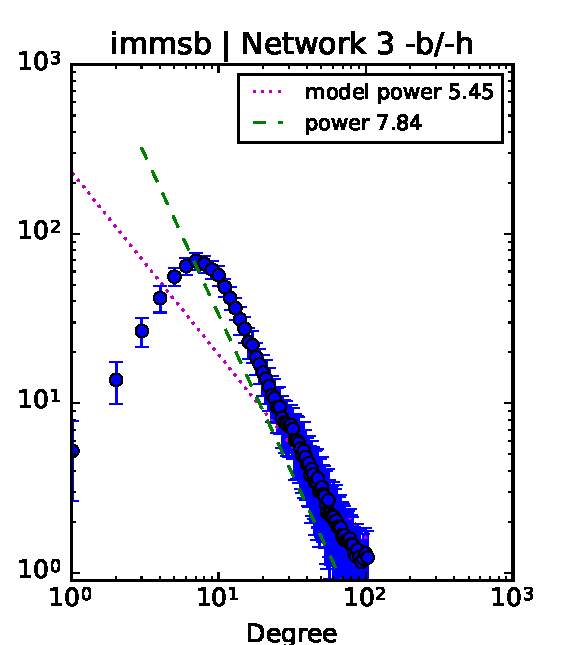
\includegraphics[scale=0.4]{img/immsb_g3_d}
	\endminipage
	\vspace{-0.4cm}
	\minipage{0.25\textwidth}
	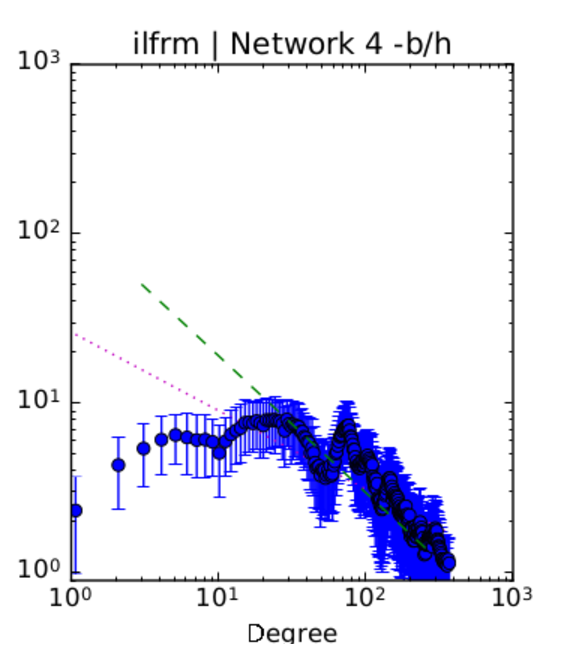
\includegraphics[scale=0.4]{img/ilfrm_g4_d}
	\endminipage
	\minipage{0.25\textwidth}
	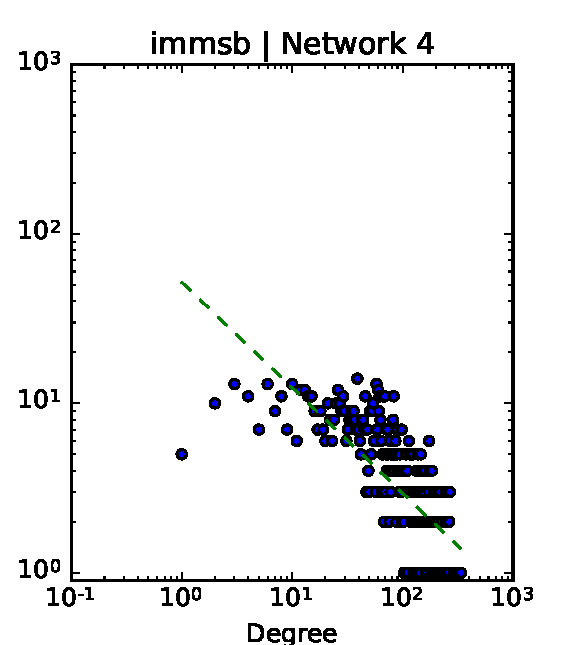
\includegraphics[scale=0.4]{img/immsb_g4_d}
	\endminipage
	
	\caption{Generated Networks with Latent Models learned from artificial datasets}
	\label{fig:gen_graph_s}
\end{figure}

\begin{figure}[h]
	\centering
	
	\minipage{0.25\textwidth}
	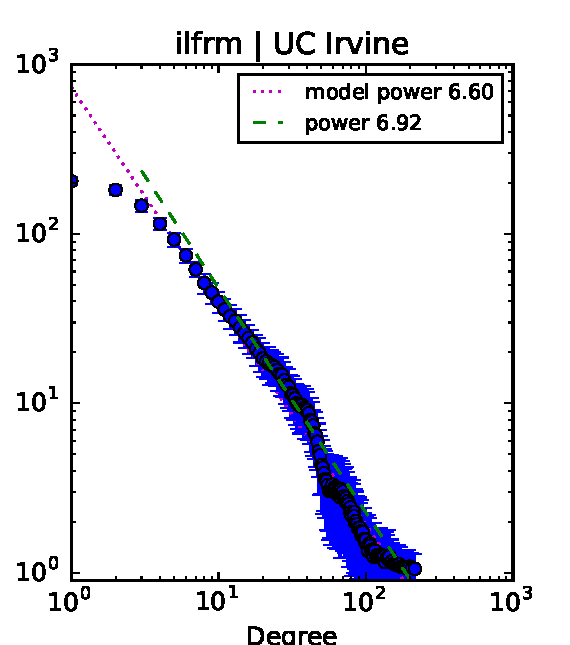
\includegraphics[scale=0.4]{img/ilfrm_irvine_d}
	\endminipage
	\minipage{0.25\textwidth}
	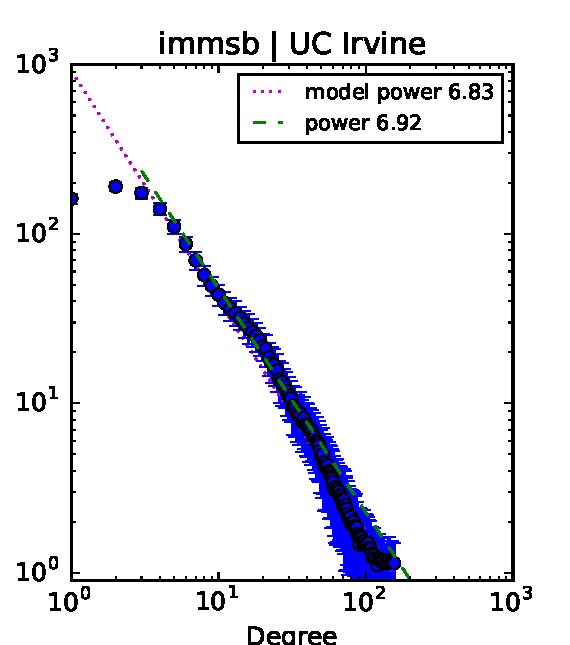
\includegraphics[scale=0.4]{img/immsb_irvine_d}
	\endminipage
	\vspace{-0.4cm}
	\minipage{0.25\textwidth}
	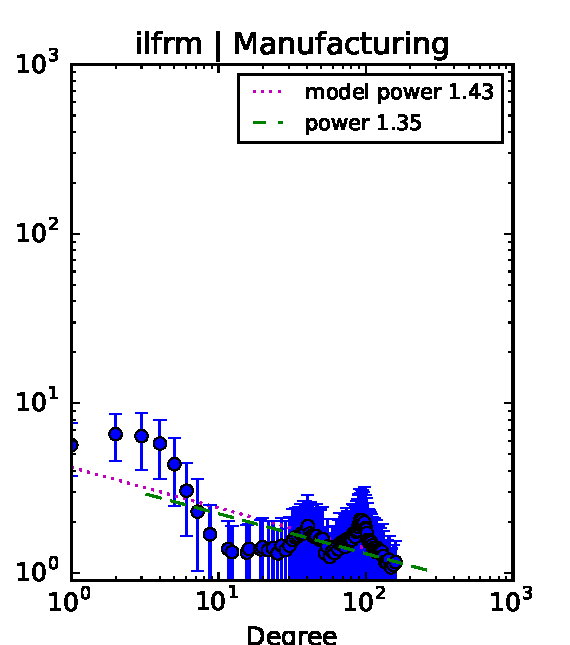
\includegraphics[scale=0.4]{img/ilfrm_manufacturing_d}
	\endminipage
	\minipage{0.25\textwidth}
	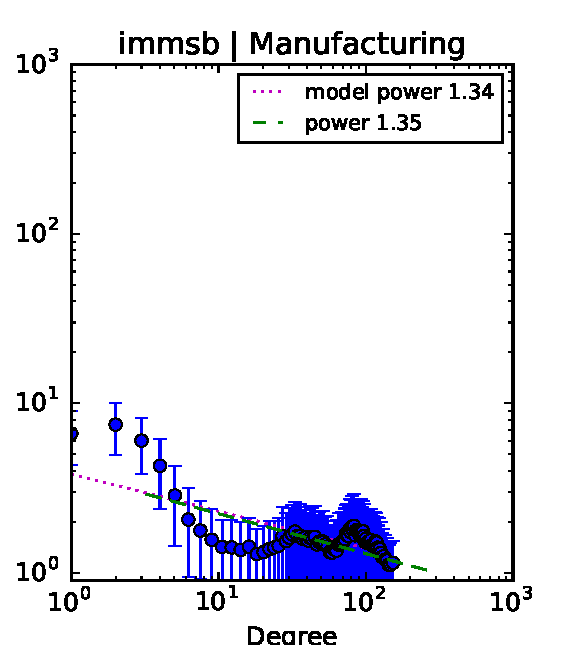
\includegraphics[scale=0.4]{img/immsb_manufacturing_d}
	\endminipage
	
	\caption{Generated Networks with Latent Models learned from artificial datasets}
	\label{fig:gen_graph_r}
\end{figure}


\begin{figure}[h]
	\centering
	
	\minipage{0.25\textwidth}
	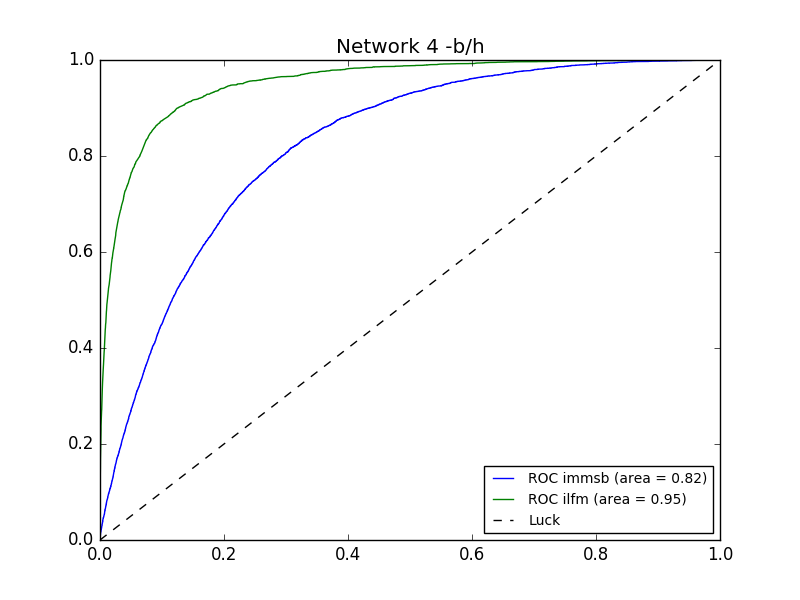
\includegraphics[scale=0.22]{img/M_e/AUC-ROC/figure_1}
	\endminipage
	\minipage{0.25\textwidth}
	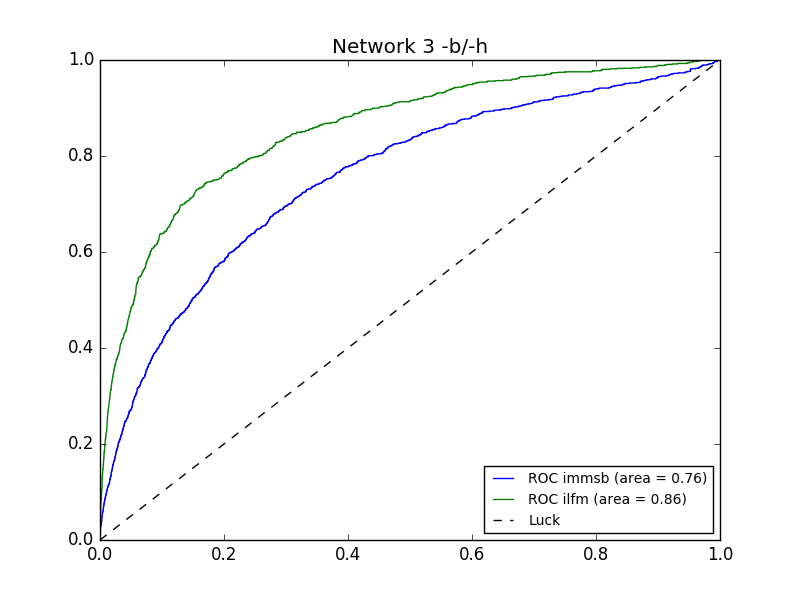
\includegraphics[scale=0.22]{img/M_e/AUC-ROC/figure_2}
	\endminipage
	\vspace{-0.4cm}
	\minipage{0.25\textwidth}
	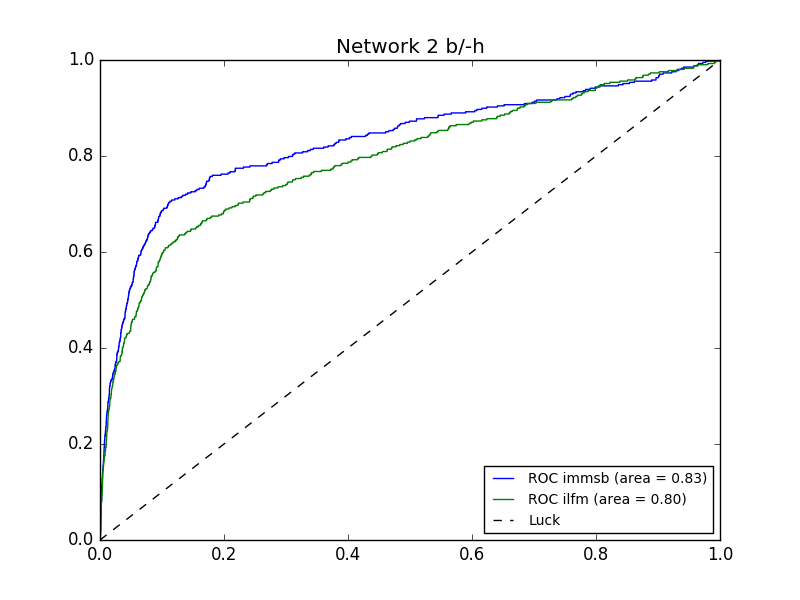
\includegraphics[scale=0.22]{img/M_e/AUC-ROC/figure_3}
	\endminipage
	\minipage{0.25\textwidth}
	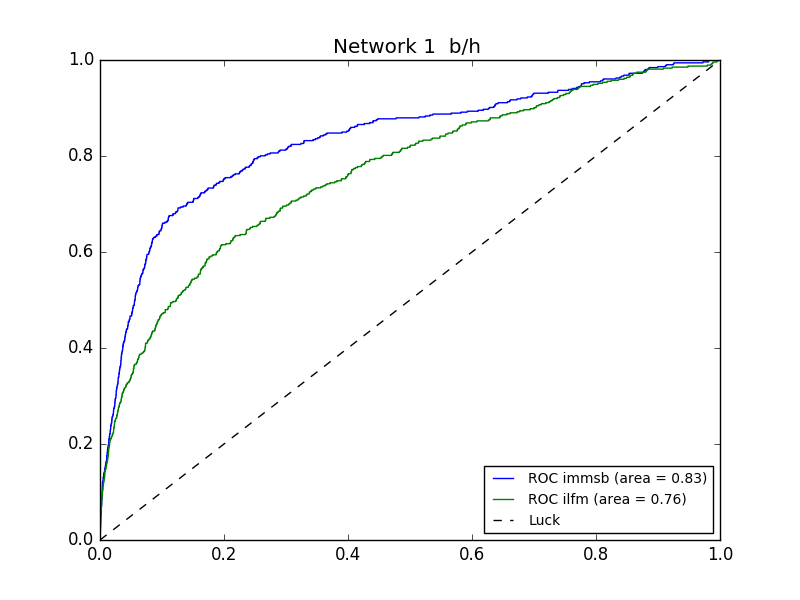
\includegraphics[scale=0.22]{img/M_e/AUC-ROC/figure_4}
	\endminipage
		\vspace{-0.4cm}
	\minipage{0.25\textwidth}
	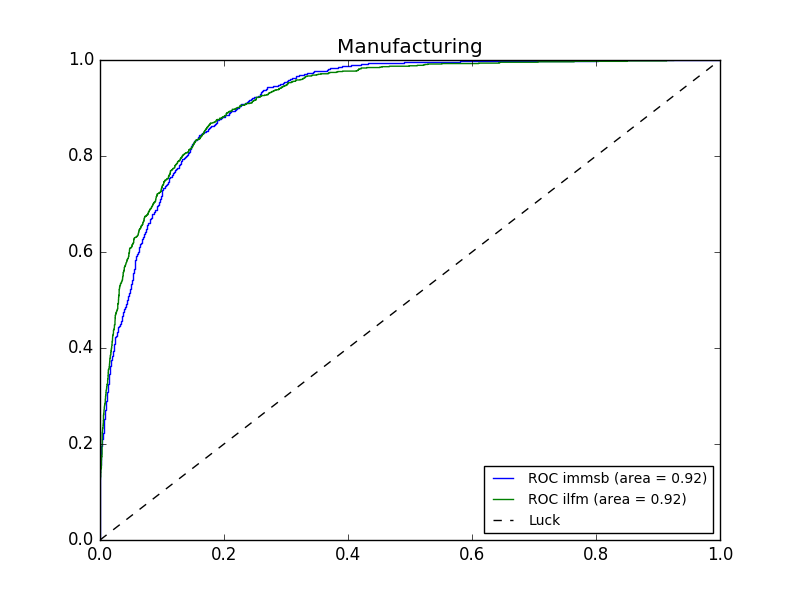
\includegraphics[scale=0.22]{img/M_e/AUC-ROC/figure_5}
	\endminipage
	\minipage{0.25\textwidth}
	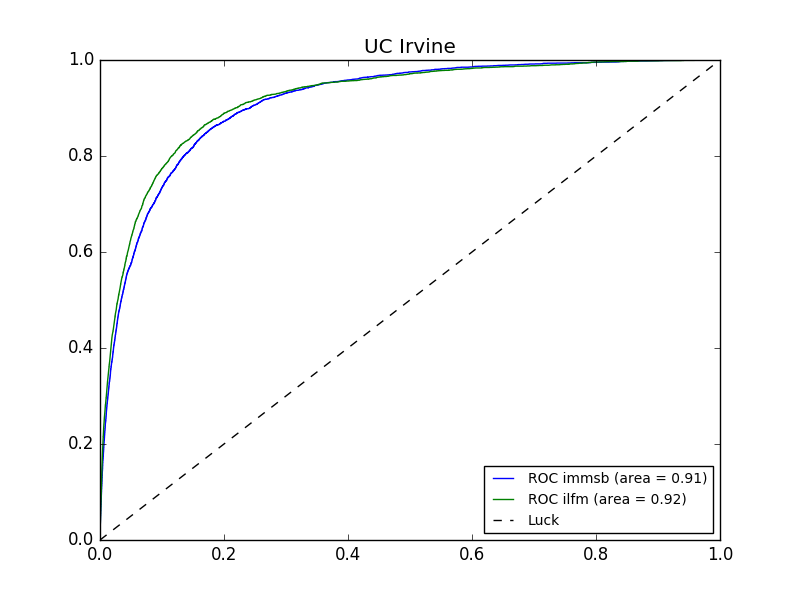
\includegraphics[scale=0.22]{img/M_e/AUC-ROC/figure_6}
	\endminipage
	
	\caption{AUC results}
	\label{fig:auc}
\end{figure}



\subsection{results}

In figure \ref{fig:gen_graph_s}, show reported the overall degree distribution for IMMSB and ILFM for the different datasets. We can see that the gap between the coefficient of the power law that fit the data in the log-log scale are shorter for the ILFM models that suggest better prediction results on average. But if we observe the result of the AUC reported in figure \ref{auc}, we see the IMMSB models has better results for all the curve measured for the network 1 and the network 2. Because those two graph are more bursty than the other, it suggest that ILFM perform better than ILFM when the networks when the preferential attachment is strongly present. Moreover, in back to figure \ref{fig:gen_graph_s}, we see that the degree distribution for IMMSB is more smooth whereas in ILFM, there is a strong variance. This is a priori to the fact that i) for ILFM  has an IPB prior which as s strong no linearity in its feature (0 or one). Thus some feature being active could impact severely on the likelihood of links. In IMMSB on the opposite the feature are smoothed by the Dirichlet distribution which has repercussions on the degree distributions. Furthermore, note that the networks where IMMSB beats ILFM, although its number of feature is almost half the number of feature for ILFM.

To conclude, these experiments show that it is important to consider a data properties based approach when evaluating and comparing the performance of learning models, and that a models that seems outperforms other in average could be non optimal depending on what we want to capture in the data.
